
\chapter{ಸಣ್ಣ ದಾರಿಯೂ ಇರದ ಜಾಗದಲ್ಲಿ ಸರ್ವೇಯ ಹೆದ್ದಾರಿ ಸಿದ್ಧವಾಯಿತು}

\vskip 7pt

ಟ್ರಿಗನಮಿಟ್ರಿಕಲ್​ ಸರ್ವೇಯ ನೆಲಗಟ್ಟಿನ ಮೇಲೆ ಇಡೀ ಇಂಡಿಯಾದ ಟೋಪೋಗ್ರಫಿಕಲ್​ ಸರ್ವೇಯನ್ನು ಆರಂಭಿಸಬೇಕಾಯಿತು. ಹೊಸದಾಗಿ ರಸ್ತೆಗಳನ್ನು, ನೀರಾವರಿ ಕಾಲುವೆಗಳನ್ನು, ರೈಲ್ವೆ ಮಾರ್ಗಗಳನ್ನು, ಹೊಸ ಜಿಲ್ಲೆಗಳ ರಚನೆಯನ್ನು ಮಾಡಬೇಕಾಯಿತು. ಮುಖ್ಯವಾಗಿ ಇಡೀ ದೇಶದ ವ್ಯವಸಾಯ ಭೂಮಿಯ ಭೂಕಂದಾಯ ನಿರ್ಧರಣೆಯನ್ನು ಮಾಡಬೇಕಾಯಿತು. ಭೂಕಂದಾಯವನ್ನು ವೈಜ್ಞಾನಿಕವಾಗಿ ನಿರ್ಧಾರ ಮಾಡಲು ರೆವಿನ್ಯೂ ಸರ್ವೇ ಮಾಡಬೇಕಾಯಿತು. ರೆವಿನ್ಯೂ ಸರ್ವೇಯ ಮುಖ್ಯ ಉದ್ದೇಶ ಆಸ್ತಿಗಳ ಮೇರೆಗಳನ್ನು, ಕಾನೂನಾತ್ಮಕ ಗಡಿ ರೇಖೆಗಳನ್ನು ನಿರ್ಧರಿಸಿ ಗ್ರಾಮವಾರು ಅವುಗಳನ್ನು ಅಳೆದು ಮ್ಯಾಪು ತಯಾರಿಸುವುದು. ಪ್ರತಿ ಗ್ರಾಮದ ಮತ್ತು ಅದರಲ್ಲಿನ ಪ್ರತಿ ಹಿಡುವಳಿಯ ಗಾತ್ರ ವಿಸ್ತೀರ್ಣ ಕಂಡು ಹಿಡಿದು, ಅದರ ವ್ಯವಸಾಯ ಉತ್ಪನ್ನ ಸಾಮರ್ಥ್ಯದ ಮೇಲೆ ಕರವನ್ನು ಹಾಕುವುದು. ಇಡೀ ದೇಶದ ರೆವಿನ್ಯೂ ಆಡಳಿತ, ಆರ್ಥಿಕ ಆಡಳಿತ ನಿಂತಿರುವುದು ಈ ರೆವಿನ್ಯೂ ಸರ್ವೇಯ ತಳಹದಿ ಮೇಲೆ. ಈ ರೆವಿನ್ಯೂ ಸರ್ವೇಯಿಂದ ವಿವಿಧ ಪ್ರಾಂತ್ಯಗಳ ಸಂಪತ್ತು, ವ್ಯವಸಾಯ ಕ್ರಮ, ಆಹಾರೋತ್ಪನ್ನ ಸಾಮರ್ಥ್ಯ ಮತ್ತು ತೆರಿಗೆಯನ್ನು ಭರಿಸುವ ಶಕ್ತಿ ಇವುಗಳ ಸ್ಪಷ್ಟ ಮಾಹಿತಿ ದೊರಕುತ್ತದೆ. ಈ ದೇಶವು ವ್ಯವಸಾಯ ಪ್ರಧಾನ ದೇಶ. ಜನರ ಒಡನಾಟ ಮತ್ತು ಅವರ ವ್ಯವಸಾಯ ಬದುಕಿನ ಆಧಾರವಾದ ಭೂಮಿಯ ಸ್ಪಷ್ಟ ಚಿತ್ರಣ ದೊರಕುವುದು ರೆವಿನ್ಯೂ ಸರ್ವೇಗಳಿಂದ. ಯಾವುದೇ ಆಡಳಿತಗಾರರಿಗೆ ಜನರ ಜೀವನೋಪಾಯವನ್ನು ಉತ್ತಮ ಪಡಿಸುವ, ದೇಶದ ಸಂಪತ್ತನ್ನು ಹೆಚ್ಚಿಸುವ ಕಾರ್ಯಕ್ಕೆ ಈ ಸರ್ವೇಗಳು ನೀಡುವ\break ಮಾಹಿತಿಗಳನ್ನು ಬಿಟ್ಟರೆ ಬೇರೆ ಆಧಾರಗಳಿಲ್ಲ. ಎಲ್ಲಾ ಅಭಿವೃದ್ಧಿ ಕಾರ್ಯಗಳನ್ನು ಯೋಜನಾಬದ್ಧವಾಗಿ ಮಾಡಲು, ಸರ್ವೇ ಮತ್ತು ಮ್ಯಾಪುಗಳು ಬೇಕೇ ಬೇಕು. ದೇಶವ್ಯಾಪಿ ಬಿಡಿ ಬಿಡಿ ಸರ್ವೇಗಳನ್ನೆಲ್ಲಾ ವೈಜ್ಞಾನಿಕವಾಗಿ ಸಮಗ್ರವಾಗಿ ಒಗ್ಗೂಡಿಸಲು ಜಿಟಿಎಸ್​ಗಳು ತಳಹದಿಯಾಗಿವೆ. ಎಲ್ಲಾ ರೀತಿಯ ಸರ್ವೇ ಮಾಡಿ ಮ್ಯಾಪ್​ ತಯಾರಿಸಿದ್ದು ಸರ್ವೇ ಆಫ್​ ಇಂಡಿಯಾ. ಈಗಿನ ಎಲ್ಲಾ ರಾಜ್ಯಗಳ ಸರ್ವೇ ಇಲಾಖೆಯ ಮಾತೃ ಸಂಸ್ಥೆ ಇದು. ಈ ನಮ್ಮ ಮ್ಯಾಪಿಂಗ್​ ಸಂಸ್ಥೆ ಸರ್ವೇ ಆಫ್​ ಇಂಡಿಯಾದ ಜನನ ಬೆಂಗಾಲ ಪ್ರಾಂತ್ಯದಲ್ಲಿ ಆಯಿತು.

\vskip 4pt

ಬ್ರಿಟೀಷರು, \enginline{1757} ರಲ್ಲಿ ಪ್ಲಾಸಿ ಕದನದ ಮೂಲಕ, ಬೆಂಗಾಲ ಪ್ರಾಂತ್ಯದಲ್ಲಿ ಮೊದಲ ಬಾರಿಗೆ, ದೇಶದ ಆಡಳಿತ ಕ್ಷೇತ್ರಕ್ಕೆ ಕಾಲಿಟ್ಟರು. ದಕ್ಷಿಣ ಭಾರತದಲ್ಲಿ, ಕರ್ನಲ್​ ಕೊಲಿನ್​ ಮೆಕೆಂಜಿ ಹಾಗು ಕರ್ನಲ್​ ವಿಲಿಯಮ್ ಲ್ಯಾಂಬ್​ಟನ್​ರವರು ತಮ್ಮ ಮ್ಯಾಪಿಂಗ್​ ಕಾರ್ಯ ಪ್ರಾರಂಭಿಸುವ ಬಹಳಷ್ಟು ಮೊದಲೇ, ಬೆಂಗಾಲದ ಪ್ರಾಂತ್ಯದಲ್ಲಿ, \enginline{1760}ರ ಸಮಯದಲ್ಲೇ ಸರ್ವೇ ಕಾರ್ಯವು ಆರಂಭವಾಗಿತ್ತು. ಬೆಂಗಾಲದ ತಮ್ಮ ಆಡಳಿತ ಪ್ರದೇಶದ ಮ್ಯಾಪಿಂಗ್​ ಕಾರ್ಯಕ್ಕೆ ಬ್ರಿಟೀಷರು ತೊಡಗಿದರು. ಇದಕ್ಕಾಗಿಯೇ, \enginline{1761}ರಲ್ಲಿ ಹ್ಯೂಗ್​ ಕ್ಯಾಮರೂನ್​ ಎಂಬುವರನ್ನು ಇಂಡಿಯಾದ ಮೊದಲ ಅಧಿಕೃತ ಸರ್ವೇಯರ್​ ಆಗಿ ನೇಮಕ ಮಾಡಲಾಗಿತ್ತು. ಈ ಕಾಲಘಟ್ಟದಲ್ಲಿಯೇ \enginline{1767}ರಲ್ಲಿ, ಬೆಂಗಾಲ ಪ್ರಾಂತ್ಯದ ಮ್ಯಾಪಿಂಗ್​ಗಾಗಿ, ‘ಸರ್ವೇ ಆಫ್​ ಇಂಡಿಯಾ’ ಸಂಸ್ಥೆಯನ್ನು ಪ್ರಾರಂಭಿಸಲಾಯಿತು. ಇತ್ತ, ಮದರಾಸು ಮತ್ತು ಮುಂಬಯಿ ಪ್ರಾಂತ್ಯಗಳೂ ಕೂಡ ಕ್ರಮೇಣವಾಗಿ ತಮ್ಮದೇ ಆದ ಸರ್ವೇ ಆಫ್​ ಇಂಡಿಯಾವನ್ನು ಸ್ಥಾಪಿಸಿಕೊಂಡಿದ್ದವು. ಅವರವರ ಪ್ರಾಂತ್ಯದ ಸರ್ವೇಗಳನ್ನು ಬಿಡಿ ಬಿಡಿಯಾಗಿ ಮಾಡಲಾಗಿತ್ತು. ಆದರೆ, ಬ್ರಿಟೀಷ್​ ಆಡಳಿತಗಾರರಿಗೆ ಸಮಗ್ರ ಬ್ರಿಟೀಷ್​ ಭಾರತದ ಮ್ಯಾಪು ಬೇಕಾಗಿತ್ತು. ಕೋಲ್ಕತ್ತಾ, ಮುಂಬಯಿ, ಮದರಾಸು ಪ್ರಾಂತ್ಯಗಳ ಸರ್ವೇ ಘಟಕಗಳ ನಡುವೆೆ ಮ್ಯಾಪಿಂಗ್​ ಮಾಹಿತಿಯ ವಿನಿಮಯ ಸಮನ್ವಯ ಕಷ್ಟಕರವಾಗಿತ್ತು. ಈ ಕಾರಣಕ್ಕೆ ಮೂರೂ ಪ್ರಾಂತ್ಯಗಳ ಸರ್ವೇ ಆಫ್​ ಇಂಡಿಯಾ ಸಂಸ್ಥೆಗಳನ್ನು ಒಗ್ಗೂಡಿಸಿ, \enginline{1815}ರಲ್ಲಿ ಏಕೀಕೃತ ಸರ್ವೇ ಆಫ್​ ಇಂಡಿಯಾವನ್ನು ರಚಿಸಲಾಯಿತು. ಆಗಿನ ಸರ್ವೇ ಆಫ್​ ಇಂಡಿಯಾದ ಕಾರ್ಯಗಳು ಪ್ರಮುಖವಾಗಿ ಮೂರು. ಅವುಗಳೆಂದರೆ, ಟ್ರಿಗನಮಿಟ್ರಿಕಲ್​ ಸರ್ವೇ, ಟೋಪೋಗ್ರಫಿಕಲ್​ ಸರ್ವೇ ಮತ್ತು ರೆವಿನ್ಯೂ ಸರ್ವೇ. ಟ್ರಿಗನಮಿಟ್ರಿಕಲ್​ ಸರ್ವೇ, ಟೋಪೋಗ್ರಫಿಕಲ್​ ಸರ್ವೇ ಮತ್ತು ರೆವಿನ್ಯೂ ಸರ್ವೇ ಕಾರ್ಯಗಳಿಗೆ ಈ ಸಂಸ್ಥೆಯೇ ಮಾತೃ ಸಂಸ್ಥೆಯಾಗಿದೆ. ಇಂದು ನಮಗೆ ಲಭ್ಯವಿರುವ ಟ್ರಿಗನಮಿಟ್ರಿಕಲ್​, ಟೋಪೋಗ್ರಫಿಕಲ್​ ಮತ್ತು ರೆವಿನ್ಯೂ ಸರ್ವೇಯ ಎಲ್ಲಾ ಮೂಲ ದಾಖಲೆಗಳೂ ಈ ಸಂಸ್ಥೆಯ ಕೊಡುಗೆಯಾಗಿದೆ. ಏಕೀಕೃತ ಮ್ಯಾಪಿಂಗ್​ ಸಂಸ್ಥೆಯ ಮೊದಲ ‘ಸರ್ವೇಯರ್​ ಜನರಲ್​ ಆಫ್​ ಇಂಡಿಯಾ’ ಆಗಿದ್ದವರು ಕರ್ನಲ್​ ಕೋಲಿನ್​ ಮೆಕೆಂಜಿಯವರು. ಕನ್ನಡ ಸಾಹಿತ್ಯ ಚರಿತ್ರೆಯಲ್ಲಿ ಮಿನುಗಿದ ಹೆಸರು ಇವರದ್ದು. ಬೆಂಗಾಲದ ಪ್ರಾಂತ್ಯದ ಆಗಿನ ಮ್ಯಾಪಿಂಗ್​ ಕಾರ್ಯದಲ್ಲಿ ಮೆಕೆಂಜೀ ಹಾಗು\break ಲ್ಯಾಂಬ್​ಟನ್​ರವರ ಮ್ಯಾಪಿಂಗ್​ ಕಾರ್ಯದಲ್ಲಿನ ಶ್ರೇಷ್ಠ ನಿಖರತೆಯ ಗುಣ ಇರಲಿಲ್ಲ. ಕರ್ನಲ್​ ಲ್ಯಾಂಬಟನ್​ರವರ ಸರ್ವೇಯೆಂದರೆ, ಇಡೀ ಭಾರತಕ್ಕೆ ಸಿಂಗಲ್​ ಫ್ರೇಮ್‌ವರ್ಕ್ ರಚನಾ ಕಾರ್ಯ. ಅದು ಉನ್ನತ ಗಣಿತ ತತ್ವದ, ಜಾಗತಿಕ ಗುಣಮಟ್ಟದ ಸರ್ವೇ ಕಾರ್ಯ.

ಬ್ರಿಟೀಷರು ತಮ್ಮ ಮ್ಯಾಪಿಂಗ್​ ಕಾರ್ಯಕ್ಕೆ ಮಹಾ ಮೇದಾವಿ ಮಿಲಿಟರಿ ಸರ್ವೇಯರುಗಳನ್ನು ಬಳಸಿಕೊಂಡಿದ್ದಾರೆ. ಸರ್ವೇಯೆಂಬ ಸಣ್ಣ ಹಾದಿಯೂ ಇಲ್ಲದ ಪರಿಸ್ಥಿತಿಯಲ್ಲಿ, ಪರಿಸರದಲ್ಲಿ ಸರ್ವೇಯ ಹೆದ್ದಾರಿಯನ್ನೇ ಆ ಮಹನೀಯ ಬ್ರಿಟೀಷ್​ ಮೇಧಾವಿ ಸರ್ವೇಯರುಗಳು ನಿರ್ಮಿಸಿ ಹೋಗಿದ್ದಾರೆ. ಸರ್ವೇಯ ರಾಜ ಮಾರ್ಗದ ಆ ನಿರ್ಮಾತೃಗಳನ್ನು ಸ್ಮರಿಸಿಕೊಳ್ಳುವುದು ಸಹ ಕೃತಜ್ಞತಾ ಕಾರ್ಯವಾಗುತ್ತದೆ. ಸರ್ವೇಯ ಆ ಮೂಲ ಪುರುಷರ ಗುಣ ಸಾಮರ್ಥ್ಯಗಳು, ಸಿದ್ಧಿ ಸಾಧನೆಗಳು ಹೆಸರು ಪ್ರಸಿದ್ಧಿಗಳು ಬಹು ಎತ್ತರದವುಗಳು, ಜಾಗತಿಕ ಮಟ್ಟದವುಗಳು.

ಮ್ಯಾಪಿಂಗ್​ ಕಾರ್ಯದಲ್ಲಿ ಗಣನೀಯ ಕೊಡುಗೆ ನೀಡಿದ ಮಹನೀಯರ ಹೆಸರುಗಳನ್ನು ಕಾಲಾನುಕ್ರಮದಲ್ಲಿ ಜೋಡಿಸಿ ನೋಡಿದರೆ ಕಾಣುವ ಮೊದಲ ಹೆಸರು ಮೇಜರ್​ ಜೇಮ್ಸ್ ರನೆಲ್​ರವರದ್ದು. ಜೇಮ್ಸ್ ರನೆಲ್​ರವರನ್ನು, ‘ಫಾದರ್​ ಆಫ್​ ಇಂಡಿಯನ್​ ಜೀಯೋಗ್ರಫಿ’ ಎಂದೇ ಕರೆಯಲಾಗುತ್ತದೆ. ಭಾರತೀಯ ಮ್ಯಾಪಿಂಗ್​ ಕ್ಷೇತ್ರದಲ್ಲಿನ ಅಪಾರ ದುಡಿಮೆಗಾಗಿ ಅವರಿಗೆ ಈ ಬಿರುದು ಸಂದಿದೆ. ಭಾರತದ ಭೌಗೋಳಿಕ ಜ್ಞಾನ ದಿಗಂತದ ವಿಸ್ತರಣೆಗೆ ಇವರ ಕೊಡುಗೆ ಅಪಾರ. ಅಷ್ಟೇ ಅಲ್ಲ, ಅವರ ಕಾಲದ ವಿಶ್ವ ಪ್ರಸಿದ್ಧ ಮ್ಯಾಪ್​ ರಚನಾಕಾರರಲ್ಲಿ\break ರೆನ್ನೆಲ್​ರವರದು ಪ್ರಮುಖ ಹೆಸರು.

ಭಾರತದಲ್ಲಿ ಮ್ಯಾಪಿಂಗ್​ ಕಾರ್ಯ ನಿರ್ವಹಿಸುವ ಮೊದಲು, ಜೇಮ್ಸ್ ರನೆಲ್​ರವರು \enginline{1756} ರಲ್ಲಿ, ಅಲ್ಪ ಪ್ರಮಾಣದ ಔಪಚಾರಿಕ ವಿದ್ಯಾಭ್ಯಾಸ ಮುಗಿಸಿ, ಅವರು \enginline{14} ವರ್ಷದವರಿದ್ದಾಗಲೇ, ‘ರಾಯಲ್​ ನೇವಿ’ ನೌಕಾ ದಳ ಸೇರುತ್ತಾರೆ. ರಾಯಲ್​ ನೇವಿ ಯೆಂದರೆ ಬ್ರಿಟನ್ನಿನ ಪ್ರಸಿದ್ಧ ಮಿಲಿಟರೀ ನೌಕಾದಳ. ರಾಯಲ್​ ನೇವಿಯಲ್ಲಿ, ಮುಂದಿನ ಏಳು ವರ್ಷಗಳು ಹಡಗಿನಲ್ಲಿ ಪ್ರಪಂಚ ಪರ್ಯಟನೆ ಮಾಡುತ್ತಾರೆ. ಕರಾವಳಿ ಮತ್ತು ಬಂದರುಗಳ ಮ್ಯಾಪಿಂಗ್​ ಕಾರ್ಯವನ್ನು ಹಡಗಿನಲ್ಲಿಯೇ ಮಾಡುತ್ತಾರೆ. ಈ ಮ್ಯಾಪಿಂಗ್​ ಕಾರ್ಯವನ್ನು ಅನೇಕ ಸಲ ಅವರು ಯುದ್ಧದ ಮಧ್ಯದಲ್ಲಿಯೆ ಮಾಡಬೇಕಾಗುತ್ತದೆೆ. ಒಂದು ಕಡೆ ಯುದ್ಧ ನಡೆಯುತ್ತಿದ್ದರೆ, ಅದರ ಜೊತೆ ಜೊತೆಗೇ ಸರ್ವೇ ಮಾಡುತ್ತಾ ಮ್ಯಾಪಿಂಗನ್ನು ಮಾಡುವ ಕಾರ್ಯ ಅವರದು.

\begin{figure}[!htbp]
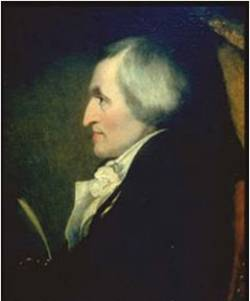
\includegraphics[scale=1.1]{"images/image017.jpg"}
\caption{ಮೇಜರ್​ ಜೇಮ್ಸ್ ರನೆಲ್​}\label{art13-fig1}
\end{figure}

ನಂತರ \enginline{1763} ರಲ್ಲಿ ರನೆಲ್​ರವರು, ಈಸ್ಟ್​ ಇಂಡಿಯಾ ಕಂಪನಿಗೆ ಸೇರಿದ ಬೆಂಗಾಲದ ಪ್ರಾಂತ್ಯದ ಸರ್ವೇಗಾಗಿ ನೇಮಕವಾಗುತ್ತಾರೆ. ರನೆಲ್​ರವರಿಗೆ ಈ ಮೊದಲು, ಕರಾವಳಿ ಮತ್ತು ಬಂದರುಗಳ ಮ್ಯಾಪಿಂಗ್​ ಕಾರ್ಯದಲ್ಲಿ ಬಹಳಷ್ಟು ಅನುಭವ ಇರುತ್ತದೆ. ಆದರೆ ಬೆಂಗಾಳದಲ್ಲಿ ಭೂ ಸರ್ವೇಯನ್ನು ಮಾಡಿ, ನಕ್ಷೆ ತಯಾರಿಸಬೇಕಾಗುತ್ತದೆ. ಸರ್ವೇಯಲ್ಲಿ ಅವರೊಂದಿಗೆ ಅನೇಕ ಜನ ದುಡಿಯುತ್ತಿದ್ದರು. ಆದರೆ ರನೆಲ್​ರವರಿಗೆ ಸರ್ವೇಯೆಂಬುದು ಒಂದು ಗೀಳು. ಅವರಿಗೆ ಅದೊಂದು ತಪಸ್ಸು. ಬೆಂಗಾಳ ಪ್ರಾಂತ್ಯದ ಸರ್ವೇಯಿಂಗ್​ ಮತ್ತು ಮ್ಯಾಪಿಂಗ್​ ಕಾರ್ಯವನ್ನು ಬಹಳಷ್ಟು ತಲೆಗೆ ಹಚ್ಚಿಕೊಂಡು, ಬಹು ಶ್ರದ್ಧೆಯಿಂದ ರನೆಲ್​ರವರು ದುಡಿದರು. ಇವರ ಕಾಲದಲ್ಲಿಯೇ ‘ಸರ್ವೇ ಆಫ್​ ಇಂಡಿಯಾ’ ಎಂಬ ಮ್ಯಾಪಿಂಗ್​ ಸಂಸ್ಥೆಯು ಪ್ರಥಮ ಬಾರಿಗೆ ಬೆಂಗಾಳ ಪ್ರಾಂತ್ಯದಲ್ಲಿ ಸ್ಥಾಪನೆಯಾಗಿದ್ದು. ಈ ಮಹಾ ಸಂಸ್ಥೆಯ ಸ್ಥಾಪನೆಗೆ ಮೇಜರ್​ ಜೇಮ್ಸ್ ರನೆಲ್​ರವರು ಬಹುಪಾಲು ಕಾರಣರಾಗಿದ್ದಾರೆ. ಆಗಿನ ಬೆಂಗಾಳದ ಗವರ್ನರ್​ ಆಗಿದ್ದ, ರಾಬರ್ಟ್ ಕ್ಲೈವ್​ರವರು, ಸರ್ವೇಯಿಂಗ್​ನಲ್ಲಿನ ಇವರ ಅಪಾರ ಆಸಕ್ತಿ, ಪ್ರತಿಭೆ ಮತ್ತು ಸಾಮರ್ಥ್ಯವನ್ನು ಕಂಡು, \enginline{1767} ರಲ್ಲಿ, ಇವರನ್ನೇ ಬೆಂಗಾಳದ ಮೊದಲ ಸರ್ವೇಯರ್​ ಜನರಲ್​ರನ್ನಾಗಿ ನೇಮಕ ಮಾಡಿದರು. ಆಗ ಇವರಿಗೆ ಕೇವಲ \enginline{24} ವರ್ಷ ವಯಸ್ಸು. ಬಂಗಾಳದ ಪ್ರಾಂತ್ಯದ, ಅಂದರೆ, ಬ್ರಿಟೀಷ್​ ಭಾರತದ ಮೊದಲ ಮ್ಯಾಪ್​, ಜೇಮ್ಸ್ ರನೆಲ್​ ಇವರಿಂದಲೇ ತಯಾರಾಯಿತು.

ರನೆಲ್​ರವರ ಕಾಲದಲ್ಲಿ ಸರ್ವೇಯಿಂಗ್​ ಚಟುವಟಿಕೆ ಈಗಿನಷ್ಟು ವಿಕಸನವಾಗಿರಲಿಲ್ಲ. ಅವರಿಗೆ ನುರಿತ ಸಿಬ್ಬಂದಿ ಸಿಗಲಿಲ್ಲ. ಸೂಕ್ತ ಉಪಕರಣವೂ ಇರಲಿಲ್ಲ. ಸಾಮಾನ್ಯ ಜನರೂ ಸರ್ವೇಯಿಂಗ್​ ಕಾರ್ಯವನ್ನು ಅನುಮಾನದಿಂದಲೇ ನೋಡುತಿದ್ದ ಕಾಲ ಅದು. ರನೆಲ್​ರವರು \enginline{1776} ರಲ್ಲಿ, ಭೂತಾನಿನ ಗಡಿಯಲ್ಲಿ, ದೂರ ಮತ್ತು ಬೇರಿಂಗ್​ಗಳನ್ನು ಅಳೆಯುವ ಕಾರ್ಯ ನಿರ್ವಹಿಸುತ್ತಿದ್ದರು. ಆ ಸಮಯದಲ್ಲಿ ರನೆಲ್​ರವರು ಕೆಲವರಿಂದ ದಾಳಿಗೆ ಒಳಗಾದರು. ಈ ದಾಳಿಯಲ್ಲಿ ರನೆಲ್​ರವರು ಗಂಭೀರವಾಗಿ ಗಾಯಗೊಂಡರು. ಜೊತೆಗೆ, ಕ್ಷೇತ್ರ ಕಾರ್ಯದ ಪ್ರತಿಕೂಲ ಪರಿಸ್ಥಿತಿಯ ಕಠಿಣ ದುಡಿಮೆಯಿಂದ ಅವರಿಗೆ ಮಲೇರಿಯಾ ಜ್ವರ ಪದೇ ಪದೇ ಬರುತಿತ್ತು. ಇದರಿಂದ ಮೊದಲಿನಂತೆ, ಕೆಲಸ ನಿರ್ವಹಿಸಲಾಗದೇ, \enginline{1777}ರಲ್ಲಿ ಅವರು ಅನಿವಾರ್ಯವಾಗಿ, ತಮ್ಮ ಸರ್ವೇಯ ಸಕ್ರಿಯ ಕ್ಷೇತ್ರ ಕಾರ್ಯದಿಂದ ನಿವೃತ್ತರಾದರು. ನಂತರ \enginline{53} ವರ್ಷಗಳು ಲಂಡನ್ನಿನಲ್ಲಿದ್ದುಕೊಂಡು, ಅನೇಕ ಮ್ಯಾಪ್​ಗಳ ರಚನಾ ಕಾರ್ಯದಲ್ಲಿ ತಮ್ಮನ್ನು ಪೂರ್ಣವಾಗಿ ತೊಡಗಿಸಿಕೊಂಡರು. ಈಸ್ಟ್​ ಇಂಡಿಯಾ ಕಂಪನಿ ಸೇವೆಯಿಂದ ನಿವೃತ್ತರಾಗಿ \enginline{6} ವರ್ಷಗಳ ನಂತರ, \enginline{1783} ರಲ್ಲಿ ಭಾರತ ಉಪಖಂಡದ ಮ್ಯಾಪನ್ನು ರಚಿಸಿದರು. ಸರ್ವೇಯೇ ಇಲ್ಲದ ಆ ಕಾಲದಲ್ಲಿ, ಸರ್ವೇ ಮಾಡಿ, ಮತ್ತು ಸರ್ವೇ ಮಾಡಿದ ಡೇಟಾ ಸಂಗ್ರಹಿಸಿ, ಅವುಗಳನ್ನು ವೈಜ್ಞಾನಿಕವಾಗಿ ಸಂಕಲಿಸಿ, ಭಾರತದ ಉಪ ಖಂಡದ ಭೌಗೋಳಿಕ ರೂಪವನ್ನು ಕಡೆದು ನಿರ್ಮಿಸಿರುವ ರನೆಲ್​ರವರ ಕಾರ್ಯ ಅನನ್ಯವಾದದ್ದು. ಈ ಮ್ಯಾಪಿಗೆ ಅವರು ‘ಮ್ಯಾಪ್​ ಆಫ್​ ಹಿಂದೂಸ್ಥಾನ್​’ ಅಥವಾ ‘ಮೊಘಲ್​ ಎಂಪೈರ್​’ ಎಂದು ಟೈಟಲ್​ ಕೊಟ್ಟಿದ್ದಾರೆ. ಇದು ರನೆಲ್​ರವರ ಬಹು ಪ್ರಸಿದ್ಧ ರಚನೆ.

ರಾಬರ್ಟ್ ಕೂಲ್​ಬ್ರೂಕ್​ \enginline{1794}ರಲ್ಲಿ, ಮೇಜರ್​ ರನೆಲ್​ರವರ ಹುದ್ದೆಗೆ ಉತ್ತರಾಧಿಕಾರಿಯಾಗಿ ಬೆಂಗಾಲದ ಸರ್ವೇಯರ್​ ಜನರಲ್​ ಆಗುತ್ತಾರೆ. ಬಂಗಾಳ ಪ್ರಾಂತ್ಯಕ್ಕೆ ಹೊಸದಾಗಿ ಸೇರಿದ ಗಂಗಾ–ಯಮುನಾ ನದಿ ಪ್ರದೇಶದಲ್ಲಿ, ನೇಪಾಳದ ಗಡಿಯ ಹಿಮಾಲಯದ ತಪ್ಪಲಿನವರೆಗಿನ ಪ್ರದೇಶಗಳನ್ನು ಮ್ಯಾಪ್​ ಮಾಡಲು ತೊಡಗುತ್ತಾರೆ. ಆದರೆ \enginline{1807–08}ರ ಅವಧಿಯಲ್ಲಿ ಇವರ ಸರ್ವೇಯಿಂದ ಬಂದ ಮ್ಯಾಪಿಂಗ್​ನಲ್ಲಿಯೂ ಸಹ, ಮೈಸೂರಿನಲ್ಲಿ ಮೆಕೆಂಜಿರವರು ನಡೆಸಿದ ಸರ್ವೇಯ ನಿಖರತೆಯ ಗುಣಗಳು ಇರಲಿಲ್ಲ. ಲ್ಯಾಂಬ್​ಟನ್​ರವರ ಸರ್ವೇಯ ಗಣಿತಾತ್ಮಕ ಗುಣವಂತೂ ಇರಲು ಸಾಧ್ಯವೇ ಇರಲಿಲ್ಲ.

ಕೂಲ್​ ಬ್ರೂಕ್​ರವರದ್ದು ರೂಟ್​ ಸರ್ವೇ. ರೂಟ್​ ಸರ್ವೇಯ ಮುಖ್ಯ ಉದ್ದೇಶವು ಯುದ್ಧ ವ್ಯವಹಾರ, ಸೈನಿಕ ಕಾರಣಕ್ಕೆ. ಸೈನಿಕರು ಸಂಚರಿಸುವ ರಸ್ತೆ, ನದಿ, ಕೋಟೆ, ಕೊತ್ತಲ, ಬೆಟ್ಟ, ಗುಡ್ಡ ಪ್ರಮುಖ ಈ ಅಂಶಗಳು ಇರುವ ಮ್ಯಾಪ್​ ತಯಾರಿಕೆ. ರೂಟ್​ ಸರ್ವೇ ಮ್ಯಾಪಿಂಗ್​ ಕಾರ್ಯದಲ್ಲಿ ಬೆಟ್ಟಗಳ ಎತ್ತರಕ್ಕಿಂತಲೂ ಬೆಟ್ಟದ ಮಧ್ಯದ ಒಳಮಾರ್ಗಗಳು ಎಲ್ಲಿವೆ. ಶತ್ರು ಸೈನ್ಯ ಎಲ್ಲಿಂದ ಒಳ ನುಸುಳಬಹುದು, ಯಾವ ಮಾರ್ಗದಲ್ಲಿ ಬ್ರಿಟೀಷ್​ ಸೈನ್ಯವು ಎದುರು ಸೈನ್ಯದ ಮೇಲೆ ದಾಳಿ ಮಾಡಬಹುದು? ಇವು ಅವರ ರೂಟ್​ ಮ್ಯಾಪ್​ನ ಮುಖ್ಯವಾದ ಉದ್ದೇಶಿತ ಅಂಶಗಳು.

